\section{Phát hiện điểm đặc trưng (Keypoint Detection)}
\label{sec:keypoint_detection}

\subsection{Giới thiệu: Tìm kiếm những "Điểm neo" trong Thế giới Thị giác}
\label{subsec:keypoint_intro}

Trong phần trước, chúng ta đã tìm hiểu cách phát hiện các cấu trúc cơ bản như đường biên. Mặc dù các đường biên rất hữu ích, chúng lại gặp phải một vấn đề cố hữu được biết đến với tên gọi \textbf{vấn đề khẩu độ (aperture problem)}. Nếu bạn chỉ nhìn vào một đoạn ngắn của một đường thẳng qua một "khẩu độ" nhỏ, bạn chỉ có thể xác định được thành phần chuyển động vuông góc với đường thẳng đó, chứ không thể xác định được chuyển động dọc theo nó. Điều này làm cho các điểm trên một đường biên trở nên không đủ tin cậy để theo dõi (tracking) một cách chính xác.

Để giải quyết vấn đề này, các nhà nghiên cứu đã tìm kiếm những điểm đặc biệt hơn trong ảnh, những điểm có cấu trúc hai chiều rõ ràng và có thể được định vị một cách không mơ hồ. Những điểm này được gọi là \textbf{điểm đặc trưng (interest points hay keypoints)}, và phổ biến nhất trong số đó là các \textbf{góc (corners)}.

\begin{center}
    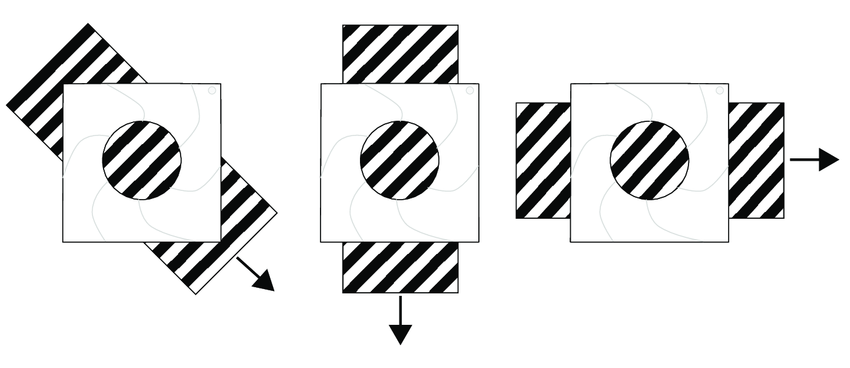
\includegraphics[width=0.8\textwidth]{images/aperture_problem.png}
    \captionof{figure}{Minh họa Vấn đề Khẩu độ (Aperture Problem). Khi chỉ quan sát một đoạn nhỏ của một đường thẳng đang di chuyển (trái), ta không thể xác định được thành phần chuyển động dọc theo đường thẳng đó. Ngược lại, khi quan sát một góc (phải), chuyển động của nó có thể được xác định một cách không mơ hồ theo cả hai chiều.}
    \label{fig:aperture_problem}
\end{center}

Một "góc" trong thị giác máy tính là một điểm mà tại đó có sự thay đổi lớn về cường độ sáng theo \textit{nhiều hướng} khác nhau. Trực giác, nếu bạn đặt một cửa sổ nhỏ xung quanh một góc và di chuyển cửa sổ đó theo bất kỳ hướng nào, nội dung bên trong cửa sổ sẽ thay đổi đáng kể. Điều này làm cho các góc trở thành những "điểm neo" lý tưởng cho các tác vụ như:
\begin{itemize}
    \item \textbf{So khớp ảnh (Image Matching):} Tìm các điểm tương ứng giữa hai hoặc nhiều ảnh của cùng một cảnh.
    \item \textbf{Theo dõi đối tượng (Object Tracking):} Theo dõi chuyển động của một đối tượng qua các khung hình video.
    \item \textbf{Tái tạo 3D (3D Reconstruction):} Sử dụng thị sai (parallax) từ các điểm tương ứng để suy ra cấu trúc 3D.
    \item \textbf{Ghép ảnh (Image Stitching / Panorama):} Tìm các điểm chung để ghép nối các ảnh lại với nhau.
\end{itemize}

Trong phần này, chúng ta sẽ khám phá các thuật toán kinh điển để phát hiện các điểm đặc trưng này, bắt đầu với hai phương pháp nền tảng dựa trên phân tích ma trận gradient: Harris và Shi-Tomasi.

\subsection{Harris Corner Detector: Tìm Góc bằng Phân tích Trị riêng}
\label{subsec:harris_corner_detector}

Thuật toán phát hiện góc Harris, được đề xuất bởi Chris Harris và Mike Stephens vào năm 1988 \cite{Harris1988}, là một trong những thuật toán phát hiện điểm đặc trưng có ảnh hưởng và được sử dụng rộng rãi nhất. Thay vì tìm kiếm các góc một cách trực tiếp, nó định lượng "tính góc" (cornerness) của mỗi pixel dựa trên một cơ sở toán học vững chắc.

\subsubsection{Trực giác: Sự thay đổi Cường độ trong Vùng lân cận}
\label{subsubsec:harris_intuition}
Ý tưởng cốt lõi của Harris là phân tích sự thay đổi của cường độ sáng khi dịch chuyển một cửa sổ nhỏ theo các hướng khác nhau.
\begin{itemize}
    \item \textbf{Vùng phẳng (Flat region):} Nếu cửa sổ nằm trên một vùng có cường độ đồng nhất, việc dịch chuyển nó theo bất kỳ hướng nào cũng sẽ không gây ra thay đổi đáng kể.
    \item \textbf{Cạnh (Edge):} Nếu cửa sổ nằm trên một cạnh, việc dịch chuyển nó \textit{dọc theo} cạnh sẽ gây ra ít thay đổi, trong khi dịch chuyển \textit{vuông góc} với cạnh sẽ gây ra thay đổi lớn.
    \item \textbf{Góc (Corner):} Nếu cửa sổ nằm trên một góc, việc dịch chuyển nó theo \textit{bất kỳ hướng nào} cũng sẽ gây ra thay đổi lớn.
\end{itemize}
Thuật toán Harris tìm cách lượng hóa sự thay đổi này. Sự thay đổi cường độ khi dịch chuyển cửa sổ một khoảng $(\Delta u, \Delta v)$ được tính bằng \textbf{Tổng các Sai số Bình phương (Sum of Squared Differences - SSD)}:
\begin{equation}
    E(\Delta u, \Delta v) = \sum_{x,y \in W} w(x, y) \left( I(x+\Delta u, y+\Delta v) - I(x, y) \right)^2
    \label{eq:ssd_harris}
\end{equation}
trong đó $W$ là cửa sổ, và $w(x, y)$ là một hàm trọng số (thường là hình chữ nhật hoặc Gaussian) để nhấn mạnh các pixel ở trung tâm.

\subsubsection{Xấp xỉ Taylor và Ma trận Cấu trúc}
\label{subsubsec:harris_taylor_approximation}
Việc tính toán trực tiếp $E(\Delta u, \Delta v)$ cho mọi $(\Delta u, \Delta v)$ là không khả thi. Thay vào đó, Harris và Stephens đã sử dụng xấp xỉ Taylor bậc nhất cho $I(x+\Delta u, y+\Delta v)$ khi $(\Delta u, \Delta v)$ là nhỏ:
\begin{equation}
    I(x+\Delta u, y+\Delta v) \approx I(x, y) + \frac{\partial I}{\partial x}\Delta u + \frac{\partial I}{\partial y}\Delta v = I(x, y) + [I_x, I_y] \begin{pmatrix} \Delta u \\ \Delta v \end{pmatrix}
\end{equation}
trong đó $I_x$ và $I_y$ là các đạo hàm riêng của ảnh theo hướng x và y (thường được tính bằng toán tử Sobel).

Thay biểu thức xấp xỉ này vào công thức SSD, ta có:
\begin{align}
    E(\Delta u, \Delta v) &\approx \sum_{x,y \in W} w(x, y) \left( I_x \Delta u + I_y \Delta v \right)^2 \\
    &= \sum_{x,y \in W} w(x, y) \left( (\Delta u, \Delta v) \begin{pmatrix} I_x \\ I_y \end{pmatrix} (I_x, I_y) \begin{pmatrix} \Delta u \\ \Delta v \end{pmatrix} \right) \\
    &= [\Delta u, \Delta v] \left( \sum_{x,y \in W} w(x, y) \begin{pmatrix} I_x^2 & I_x I_y \\ I_x I_y & I_y^2 \end{pmatrix} \right) \begin{pmatrix} \Delta u \\ \Delta v \end{pmatrix} \\
    &= [\Delta u, \Delta v] \mathbf{M} \begin{pmatrix} \Delta u \\ \Delta v \end{pmatrix}
\end{align}
Ma trận $\mathbf{M}$ là một ma trận đối xứng $2 \times 2$ được gọi là \textbf{ma trận cấu trúc (structure tensor)} hoặc ma trận tự tương quan (autocorrelation matrix):
\begin{equation}
    \mathbf{M} = \sum_{x,y \in W} w(x, y) \begin{pmatrix} I_x^2 & I_x I_y \\ I_x I_y & I_y^2 \end{pmatrix} = \begin{pmatrix} \sum wI_x^2 & \sum wI_x I_y \\ \sum wI_x I_y & \sum wI_y^2 \end{pmatrix}
    \label{eq:harris_matrix_m}
\end{equation}
Lưu ý rằng các tổng này được tính trên toàn bộ cửa sổ $W$ xung quanh pixel đang xét.

\subsubsection{Phân tích Trị riêng của Ma trận M}
\label{subsubsec:harris_eigen_analysis}
Biểu thức $E(\Delta u, \Delta v) \approx [\Delta u, \Delta v] \mathbf{M} [\Delta u, \Delta v]^T$ mô tả một hình elip trong không gian dịch chuyển $(\Delta u, \Delta v)$. Các trị riêng (eigenvalues) $\lambda_1, \lambda_2$ và các vector riêng (eigenvectors) tương ứng của ma trận $\mathbf{M}$ mô tả hình dạng và hướng của elip này. Cụ thể, các trị riêng cho biết độ lớn của sự thay đổi cường độ theo hai hướng chính (vuông góc với nhau) được chỉ ra bởi các vector riêng.
\begin{itemize}
    \item \textbf{Vùng phẳng:} $I_x$ và $I_y$ đều nhỏ trong cửa sổ $W$. Ma trận $\mathbf{M}$ sẽ có các phần tử gần 0. Cả hai trị riêng $\lambda_1, \lambda_2$ đều nhỏ.
    \item \textbf{Cạnh:} Có một hướng gradient chính. Ví dụ, với một cạnh ngang, $I_y$ sẽ lớn và $I_x$ sẽ nhỏ. Ma trận $\mathbf{M}$ sẽ có $\sum wI_y^2$ lớn, trong khi các phần tử khác nhỏ. Do đó, một trị riêng sẽ rất lớn và trị riêng còn lại sẽ rất nhỏ ($\lambda_1 \gg \lambda_2 \approx 0$).
    \item \textbf{Góc:} Gradient có độ lớn theo nhiều hướng. $I_x$ và $I_y$ đều lớn và thay đổi hướng trong cửa sổ. Cả hai trị riêng $\lambda_1, \lambda_2$ đều lớn.
\end{itemize}

\begin{center}
    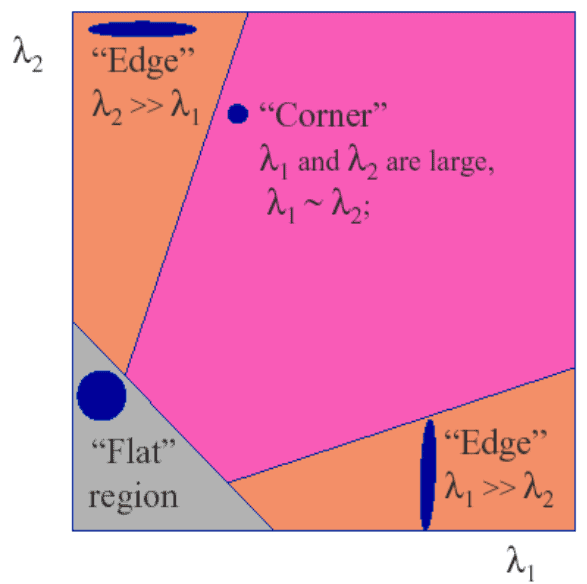
\includegraphics[width=0.9\textwidth]{images/harris_eigen_visualization.png}
    \captionof{figure}{Mối liên hệ giữa loại vùng ảnh và các trị riêng của ma trận cấu trúc M. Elip biểu diễn sự thay đổi $E(\Delta u, \Delta v)$. Vùng phẳng có cả hai trị riêng nhỏ. Cạnh có một trị riêng lớn và một trị riêng nhỏ. Góc có cả hai trị riêng đều lớn.}
    \label{fig:harris_eigen_viz}
\end{center}

\subsubsection{Hàm phản hồi ''Cornerness''}
\label{subsubsec:harris_response_function}
Việc tính toán trực tiếp các trị riêng cho mỗi pixel là tốn kém. Thay vào đó, Harris và Stephens đề xuất một hàm phản hồi $R$ có thể được tính toán trực tiếp từ các phần tử của ma trận $\mathbf{M}$ mà không cần phân rã trị riêng:
\begin{equation}
    R = \det(\mathbf{M}) - k \cdot (\text{trace}(\mathbf{M}))^2
    \label{eq:harris_response_r}
\end{equation}
trong đó:
\begin{itemize}
    \item $\det(\mathbf{M}) = \lambda_1 \lambda_2 = (\sum wI_x^2)(\sum wI_y^2) - (\sum wI_x I_y)^2$
    \item $\text{trace}(\mathbf{M}) = \lambda_1 + \lambda_2 = \sum wI_x^2 + \sum wI_y^2$
    \item $k$ là một hằng số thực nghiệm, thường trong khoảng $[0.04, 0.06]$.
\end{itemize}

Phân tích giá trị của $R$ dựa trên các trị riêng:
\begin{itemize}
    \item \textbf{Vùng phẳng:} $\lambda_1, \lambda_2$ nhỏ $\implies R$ nhỏ.
    \item \textbf{Cạnh:} Một trị riêng lớn hơn nhiều trị riêng còn lại ($\lambda_1 \gg \lambda_2 \approx 0$) $\implies \det(\mathbf{M}) \approx 0$ và $\text{trace}(\mathbf{M})$ lớn $\implies R < 0$.
    \item \textbf{Góc:} $\lambda_1, \lambda_2$ đều lớn và có giá trị tương đương $\implies \det(\mathbf{M})$ lớn và $\text{trace}(\mathbf{M})$ lớn, nhưng $\det(\mathbf{M})$ lớn hơn $k \cdot (\text{trace}(\mathbf{M}))^2$ $\implies R$ lớn và dương.
\end{itemize}

Vậy, quy trình phát hiện góc Harris là: tính giá trị $R$ cho mỗi pixel. Các pixel có giá trị $R$ lớn và dương là các ứng cử viên cho điểm góc.

\subsubsection{Các bước Hoàn chỉnh của Thuật toán Harris}
\label{subsubsec:harris_full_algorithm}
\begin{enumerate}
    \item Tính đạo hàm ảnh $I_x, I_y$ trên toàn bộ ảnh.
    \item Tính ba thành phần của ma trận $\mathbf{M}$ tại mỗi pixel: $I_x^2, I_y^2, I_x I_y$.
    \item Áp dụng một bộ lọc tổng (ví dụ, Gaussian hoặc hộp) lên ba ảnh này để tính các tổng $\sum wI_x^2, \sum wI_y^2, \sum wI_x I_y$ trong cửa sổ $W$ cho mỗi pixel.
    \item Tính toán giá trị phản hồi cornerness $R$ cho mỗi pixel.
    \item Áp dụng một ngưỡng lên bản đồ phản hồi $R$ để giữ lại các điểm có khả năng là góc.
    \item Áp dụng \textbf{Non-Maximum Suppression} để tìm các cực đại cục bộ trong bản đồ phản hồi, đảm bảo mỗi góc chỉ được phát hiện một lần.
\end{enumerate}

\subsection{Shi-Tomasi Corner Detector ("Good Features to Track")}
\label{subsec:shi_tomasi}

Năm 1994, Jianbo Shi và Carlo Tomasi đã đề xuất một cải tiến nhỏ nhưng rất quan trọng cho thuật toán Harris trong bài báo nổi tiếng "Good Features to Track" \cite{Shi1994}. Họ đã phân tích lại tiêu chí lựa chọn đặc trưng từ góc độ của sự ổn định khi theo dõi (tracking).

\subsubsection{Một Tiêu chí Đơn giản hơn}
\label{subsubsec:shi_tomasi_criterion}
Shi và Tomasi chỉ ra rằng một đặc trưng tốt để theo dõi là một đặc trưng mà ma trận cấu trúc $\mathbf{M}$ của nó "well-conditioned", tức là không quá chênh lệch giữa các trị riêng. Điều này có nghĩa là cả hai trị riêng $\lambda_1, \lambda_2$ đều phải đủ lớn.

Thay vì sử dụng hàm phản hồi $R$ phức tạp của Harris, họ đề xuất một tiêu chí đơn giản hơn nhiều:
\begin{equation}
    R_{\text{Shi-Tomasi}} = \min(\lambda_1, \lambda_2)
    \label{eq:shi_tomasi_response}
\end{equation}
Một pixel được coi là một "good feature" nếu $R_{\text{Shi-Tomasi}}$ của nó lớn hơn một ngưỡng cho trước.
\begin{equation}
    \min(\lambda_1, \lambda_2) > \lambda_{\text{threshold}}
\end{equation}

\subsubsection{So sánh với Harris}
\label{subsubsec:shi_tomasi_vs_harris}
\begin{itemize}
    \item \textbf{Về mặt lý thuyết:} Tiêu chí của Shi-Tomasi trực tiếp hơn. Nó đảm bảo rằng không có hướng nào mà sự thay đổi cường độ lại quá yếu, điều này rất quan trọng cho sự ổn định của các thuật toán theo dõi dựa trên gradient như Lucas-Kanade. Trong khi đó, hàm $R$ của Harris có thể cho giá trị cao ngay cả khi một trong hai trị riêng khá nhỏ (miễn là trị riêng còn lại đủ lớn để bù lại).
    \item \textbf{Về mặt thực tế:} Thuật toán Shi-Tomasi có xu hướng chọn ra các góc rõ ràng và phân bố đều hơn. Các điểm được chọn thường ổn định hơn khi theo dõi qua nhiều khung hình. Do đó, nó đã trở thành lựa chọn mặc định trong nhiều ứng dụng theo dõi đặc trưng, ví dụ như trong thư viện OpenCV.
\end{itemize}

\begin{center}
    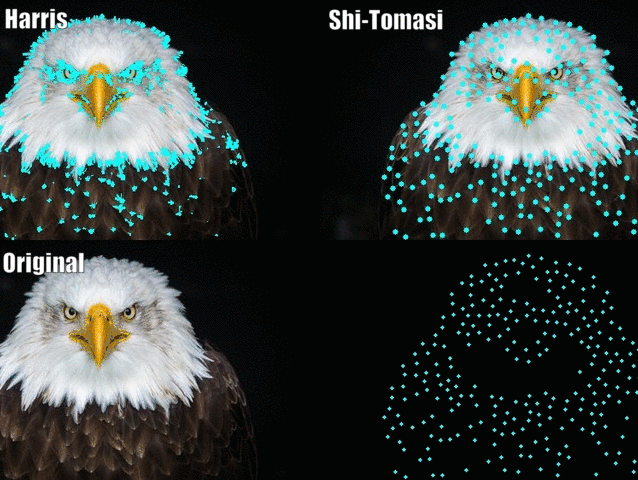
\includegraphics[width=0.9\textwidth]{images/harris_vs_shi_tomasi.png}
    \captionof{figure}{So sánh các điểm đặc trưng được phát hiện bởi Harris (trái) và Shi-Tomasi (phải) trên cùng một ảnh. Thuật toán Shi-Tomasi thường loại bỏ các điểm kém ổn định hơn và cho kết quả "sạch" hơn, phù hợp cho các tác vụ theo dõi.}
    \label{fig:harris_vs_shi_tomasi_example}
\end{center}

Mặc dù tiêu chí của Shi-Tomasi yêu cầu tính toán trực tiếp các trị riêng, nhưng đối với ma trận $2 \times 2$, việc này có thể được thực hiện hiệu quả thông qua một công thức giải phương trình bậc hai, không tốn kém hơn đáng kể so với việc tính toán hàm $R$ của Harris.

\subsubsection{Ví dụ Mã nguồn với OpenCV}
\label{subsubsec:harris_shi_tomasi_code}
OpenCV cung cấp hàm `goodFeaturesToTrack` để triển khai thuật toán Shi-Tomasi (và có thể được cấu hình để dùng Harris).

\begin{minted}[fontsize=\footnotesize, frame=single, linenos=true]{python}
import cv2
import numpy as np
import matplotlib.pyplot as plt

try:
    # Tải ảnh và chuyển sang ảnh xám
    image = cv2.imread('chessboard.png')
    if image is None:
        raise FileNotFoundError("Image not found. Please provide a sample image 'chessboard.png'")
        
    gray_image = cv2.cvtColor(image, cv2.COLOR_BGR2GRAY)
    
    # --- Harris Corner Detector ---
    # cv2.cornerHarris(image, blockSize, ksize, k)
    # blockSize: Kích thước cửa sổ để tính ma trận M
    # ksize: Kích thước của kernel Sobel
    # k: Hằng số Harris
    harris_response = cv2.cornerHarris(gray_image, blockSize=2, ksize=3, k=0.04)
    
    # Để trực quan hóa, ta có thể giãn nở kết quả để các điểm góc rõ hơn
    harris_response_dilated = cv2.dilate(harris_response, None)
    
    # Vẽ các điểm góc tìm được lên ảnh gốc
    image_harris = image.copy()
    # Đặt ngưỡng để chọn các điểm có phản hồi cao
    image_harris[harris_response_dilated > 0.01 * harris_response_dilated.max()] = [0, 0, 255] # Màu đỏ

    # --- Shi-Tomasi Corner Detector ("Good Features to Track") ---
    # cv2.goodFeaturesToTrack(image, maxCorners, qualityLevel, minDistance)
    # maxCorners: Số lượng góc tốt nhất cần tìm.
    # qualityLevel: Ngưỡng chất lượng (0-1). Một góc có chất lượng C sẽ bị loại nếu có góc tốt hơn với chất lượng C' > C trong vùng lân cận.
    # minDistance: Khoảng cách Euclid tối thiểu giữa các góc được trả về.
    corners_shi_tomasi = cv2.goodFeaturesToTrack(gray_image, maxCorners=100, qualityLevel=0.01, minDistance=10)
    corners_shi_tomasi = np.int0(corners_shi_tomasi)
    
    image_shi_tomasi = image.copy()
    for i in corners_shi_tomasi:
        x, y = i.ravel()
        cv2.circle(image_shi_tomasi, (x, y), 3, (0, 255, 0), -1) # Màu xanh lá

    # Hiển thị kết quả
    fig, axs = plt.subplots(1, 2, figsize=(12, 6))
    axs[0].imshow(cv2.cvtColor(image_harris, cv2.COLOR_BGR2RGB))
    axs[0].set_title('Harris Corner Detector')
    axs[0].axis('off')
    
    axs[1].imshow(cv2.cvtColor(image_shi_tomasi, cv2.COLOR_BGR2RGB))
    axs[1].set_title('Shi-Tomasi "Good Features to Track"')
    axs[1].axis('off')
    
    plt.tight_layout()
    plt.show()

except FileNotFoundError as e:
    print(e)
\end{minted}

Đoạn mã trên cho thấy cách triển khai và sự khác biệt trong giao diện của hai thuật toán trong OpenCV. Thuật toán Harris trả về một bản đồ phản hồi trên toàn bộ ảnh, đòi hỏi người dùng phải tự xử lý ngưỡng và non-maximum suppression. Trong khi đó, `goodFeaturesToTrack` thực hiện tất cả các bước này và trực tiếp trả về một danh sách các điểm góc tốt nhất, làm cho nó tiện lợi hơn cho các ứng dụng thực tế.

\subsection{FAST (Features from Accelerated Segment Test)}
\label{subsec:fast_detector}

Các thuật toán Harris và Shi-Tomasi, mặc dù mạnh mẽ, nhưng lại khá tốn kém về mặt tính toán vì chúng đòi hỏi các phép tính đạo hàm và tích chập trên các vùng lân cận. Đối với các ứng dụng thời gian thực như SLAM (Simultaneous Localization and Mapping) trên robot di động, một phương pháp nhanh hơn là cần thiết. FAST, được đề xuất bởi Rosten và Drummond vào năm 2006 \cite{Rosten2006}, đã ra đời để đáp ứng nhu cầu này.

\subsubsection{Trực giác: Kiểm tra Vòng tròn Pixel}
\label{subsubsec:fast_intuition}
Thay vì tính toán gradient, FAST hoạt động dựa trên một ý tưởng rất đơn giản:
\begin{quote}
    Một pixel $p$ là một điểm góc nếu tồn tại một cung gồm $N$ pixel liên tiếp trên một vòng tròn gồm 16 pixel xung quanh $p$, mà tất cả các pixel trên cung đó đều sáng hơn hoặc tối hơn $p$ một ngưỡng $t$ nhất định.
\end{quote}
Vòng tròn này là một phiên bản rời rạc của vòng tròn Bresenham có bán kính 3 pixel.

\begin{center}
    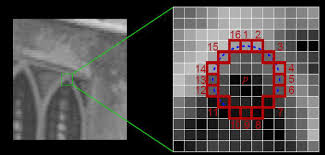
\includegraphics[width=0.7\textwidth]{images/fast_bresenham_circle.jpg}
    \captionof{figure}{Nguyên lý hoạt động của FAST. (Trái) Pixel ứng viên $p$ và 16 pixel lân cận trên vòng tròn Bresenham. (Phải) Sơ đồ 16 pixel được đánh số. Thuật toán kiểm tra xem có một cung gồm $N$ (thường là 9 hoặc 12) pixel liên tiếp đều sáng hơn $I_p + t$ hoặc tối hơn $I_p - t$.}
    \label{fig:fast_circle}
\end{center}

\subsubsection{Thuật toán và Tối ưu hóa Tốc độ}
\label{subsubsec:fast_algorithm_optimization}
Thuật toán cơ bản như sau:
\begin{enumerate}
    \item Chọn một pixel ứng viên $p$ với cường độ $I_p$.
    \item Chọn một ngưỡng cường độ $t$.
    \item Xét 16 pixel trên vòng tròn bán kính 3 xung quanh $p$.
    \item Một pixel $x$ trên vòng tròn được coi là "sáng hơn" nếu $I_x > I_p + t$, "tối hơn" nếu $I_x < I_p - t$, hoặc "tương tự".
    \item Nếu tồn tại một cung gồm $N$ pixel liên tiếp đều "sáng hơn" hoặc đều "tối hơn", thì $p$ được đánh dấu là một điểm góc. Giá trị $N$ thường được chọn là 12 hoặc 9.
\end{enumerate}

Để làm cho thuật toán cực kỳ nhanh, Rosten và Drummond đã đề xuất một bài kiểm tra tốc độ cao:
\begin{description}
    \item[High-speed test:] Chỉ kiểm tra 4 pixel tại các vị trí 1, 5, 9, và 13 (các điểm trên trục ngang và dọc). Nếu $p$ là một góc, thì ít nhất 3 trong số 4 pixel này phải thỏa mãn điều kiện ngưỡng. Nếu điều kiện này không được đáp ứng, $p$ chắc chắn không phải là góc và có thể bị loại bỏ ngay lập tức. Bài kiểm tra đơn giản này giúp loại bỏ phần lớn các pixel không phải góc một cách cực nhanh.
\end{description}
Chỉ những pixel vượt qua bài kiểm tra tốc độ cao này mới được kiểm tra đầy đủ trên tất cả 16 pixel.

\subsubsection{Học máy để Tối ưu hóa}
\label{subsubsec:fast_machine_learning}
Một trong những cải tiến quan trọng của FAST là việc sử dụng học máy để tạo ra một bộ phát hiện còn nhanh hơn nữa.
\begin{enumerate}
    \item \textbf{Thu thập dữ liệu huấn luyện:} Chạy thuật toán FAST trên một tập hợp lớn các ảnh và lưu lại trạng thái (sáng hơn, tối hơn, tương tự) của 16 pixel lân cận cho mọi điểm góc đã phát hiện.
    \item \textbf{Xây dựng cây quyết định:} Sử dụng một thuật toán học cây quyết định như ID3. Thuật toán này sẽ học cách chọn ra một chuỗi các pixel để kiểm tra sao cho có thể phân loại một điểm là "góc" hay "không phải góc" với ít lần kiểm tra nhất. Cây quyết định học được này tối ưu hóa thứ tự truy cập các pixel.
    \item \textbf{Tạo mã nguồn:} Cây quyết định học được sau đó có thể được biên dịch trực tiếp thành mã nguồn C hoặc assembly, tạo ra một bộ phát hiện cực kỳ nhanh và hiệu quả.
\end{enumerate}
Phiên bản này được gọi là FAST-ER (FAST-Enhanced Repeatability) \cite{Rosten2010}, cho thấy hiệu suất vượt trội.

\subsubsection{Non-maximal Suppression cho FAST}
\label{subsubsec:fast_nms}
FAST có xu hướng phát hiện các điểm góc nằm gần nhau. Để giải quyết vấn đề này, cần phải áp dụng Non-maximal Suppression. Tuy nhiên, bản thân FAST không định nghĩa một hàm phản hồi "cornerness" như Harris. Một hàm điểm số (score function) $V$ được định nghĩa cho mỗi điểm góc đã phát hiện:
\begin{equation}
    V = \max \left( \sum_{x \in S_{\text{bright}}} |I_x - I_p|, \sum_{x \in S_{\text{dark}}} |I_p - I_x| \right)
\end{equation}
Trong đó $S_{\text{bright}}$ và $S_{\text{dark}}$ là các tập hợp pixel trên cung liên tiếp sáng hơn hoặc tối hơn $p$. Sau khi tính $V$ cho tất cả các điểm góc, các điểm không phải là cực đại cục bộ trong một vùng lân cận sẽ bị loại bỏ.

\subsection{So sánh và Ứng dụng}
\label{subsec:keypoint_comparison_applications}

\subsubsection{So sánh Hiệu năng}
\label{subsubsec:detector_performance_comparison}
Harris, Shi-Tomasi, và FAST là ba trong số những bộ phát hiện điểm đặc trưng quan trọng nhất. Mỗi loại có những ưu và nhược điểm riêng.

\begin{table}[h!]
    \centering
    \caption{So sánh các thuật toán phát hiện điểm đặc trưng}
    \label{tab:detector_comparison}
    \begin{tabular}{|l|p{4cm}|p{4cm}|p{4cm}|}
        \hline
        \textbf{Tiêu chí} & \textbf{Harris / Shi-Tomasi} & \textbf{FAST} \\
        \hline
        \textbf{Nguyên lý} & Dựa trên đạo hàm (gradient) của ảnh, phân tích ma trận cấu trúc. & Dựa trên so sánh cường độ của các pixel trên một vòng tròn. \\
        \hline
        \textbf{Tốc độ} & Tương đối chậm. Đòi hỏi các phép tính đạo hàm, tích chập, và có thể là trị riêng. & Rất nhanh. Chỉ bao gồm các phép so sánh số nguyên. Được tối ưu hóa cho các ứng dụng thời gian thực. \\
        \hline
        \textbf{Độ chính xác} & Cao. Các điểm góc được định vị với độ chính xác cao. Có thể dễ dàng mở rộng để đạt độ chính xác dưới pixel (sub-pixel). & Thấp hơn. Vị trí của góc có thể không chính xác bằng, đặc biệt trên các cấu trúc không phải là góc "sắc nét" lý tưởng. \\
        \hline
        \textbf{Độ lặp lại (Repeatability)} & Tốt. Đặc biệt là Shi-Tomasi. Tương đối ổn định dưới sự thay đổi ánh sáng và góc nhìn nhỏ. & Tốt, nhưng nhạy cảm hơn với nhiễu ở mức độ cao. \\
        \hline
        \textbf{Tính bất biến với xoay} & Có tính bất biến với xoay do phân tích trị riêng là bất biến. & Không có tính bất biến với xoay về mặt lý thuyết. Mẫu pixel trên vòng tròn sẽ thay đổi khi ảnh bị xoay. \\
        \hline
        \textbf{Hàm phản hồi "Cornerness"} & Có (R của Harris, hoặc $\min(\lambda_1, \lambda_2)$ của Shi-Tomasi). & Không có một cách tự nhiên. Cần định nghĩa một hàm điểm số riêng cho NMS. \\
        \hline
    \end{tabular}
\end{table}

\textbf{Kết luận:}
\begin{itemize}
    \item Nếu \textbf{độ chính xác và độ ổn định} là ưu tiên hàng đầu (ví dụ: trong các ứng dụng offline như tái tạo 3D, ghép ảnh), \textbf{Shi-Tomasi} là một lựa chọn tuyệt vời.
    \item Nếu \textbf{tốc độ} là yếu tố quan trọng nhất (ví dụ: SLAM thời gian thực trên các thiết bị có tài nguyên hạn chế), \textbf{FAST} là lựa chọn không thể thay thế.
\end{itemize}
Trong thực tế, nhiều hệ thống hiện đại sử dụng kết hợp các phương pháp. Ví dụ, thuật toán ORB (sẽ được thảo luận trong phần sau) sử dụng FAST để phát hiện các điểm đặc trưng một cách nhanh chóng, sau đó sử dụng một biến thể của Harris để xếp hạng và lọc chúng.

\subsubsection{Ứng dụng trong So khớp và Theo dõi}
\label{subsubsec:keypoint_matching_tracking_apps}
Phát hiện điểm đặc trưng là bước đầu tiên trong một pipeline lớn hơn. Sau khi phát hiện, các bước tiếp theo thường là:
\begin{enumerate}
    \item \textbf{Trích xuất Bộ mô tả (Descriptor Extraction):} Đối với mỗi điểm đặc trưng, một vùng lân cận (patch) xung quanh nó được xử lý để tạo ra một vector đặc trưng (bộ mô tả). Vector này cần phải có tính phân biệt cao. Chúng ta sẽ tìm hiểu kỹ về các bộ mô tả như SIFT, SURF, ORB trong phần tiếp theo.
    \item \textbf{So khớp (Matching):} Với hai ảnh, chúng ta phát hiện và mô tả các điểm đặc trưng trên cả hai. Sau đó, đối với mỗi điểm đặc trưng ở ảnh thứ nhất, chúng ta tìm điểm đặc trưng ở ảnh thứ hai có bộ mô tả gần nhất (ví dụ, theo khoảng cách Euclid).
    \item \textbf{Theo dõi (Tracking):} Trong một video, thay vì thực hiện so khớp độc lập giữa mỗi cặp khung hình, chúng ta có thể sử dụng các thuật toán theo dõi hiệu quả hơn như \textbf{Lucas-Kanade Optical Flow}. Thuật toán này, một khi đã xác định được một tập hợp các đặc trưng tốt (ví dụ, bằng Shi-Tomasi) ở khung hình đầu tiên, sẽ cố gắng theo dõi vị trí của chúng ở các khung hình tiếp theo bằng cách giải một bài toán tối ưu hóa nhỏ dựa trên giả định rằng chuyển động là nhỏ.
\end{enumerate}

\section*{Tài liệu tham khảo}
\begin{itemize}
    \item[1] Harris, C.; Stephens, M. A Combined Corner and Edge Detector. In \textit{Proceedings of the 4th Alvey Vision Conference}, 1988.
    \item[2] Shi, J.; Tomasi, C. Good Features to Track. In \textit{Proceedings of the IEEE Conference on Computer Vision and Pattern Recognition (CVPR)}, 1994.
    \item[3] Rosten, E.; Drummond, T. Machine learning for high-speed corner detection. In \textit{European Conference on Computer Vision (ECCV)}, 2006.
    \item[4] Rosten, E.; Porter, R.; Drummond, T. FASTER and better: a machine learning approach to corner detection. \textit{IEEE Transactions on Pattern Analysis and Machine Intelligence} \textbf{2010}, \textit{32}(1), 105-119.
    \item[5] Sánchez, J.; Monzón, N.; Salgado, A. An Analysis and Implementation of the Harris Corner Detector. \textit{Image Processing On Line} \textbf{2018}, \textit{8}, 305-328.
    \item[6] Karami, E.; Prasad, S.; Shehata, M. Image Matching Using SIFT, SURF, BRIEF and ORB: Performance Comparison for Distorted Images. \textit{arXiv preprint arXiv:1710.02726}, 2017.
\end{itemize}
